\section{Supervisión de servidor web (HTTP)}
\subsection{Instalación}
Para la supervisión del funcionamiento de este servidor, se realizó primero la instalación que es muy sencilla en una máquina virtual Ubuntu Server, en la cual se ingresó el comando \textbf{sudo apt-get install apache2}, mostrado en la figura \ref{image:http1} mismo que instalaba las librerías necesarias de este servidor.

\FloatBarrier
\begin{figure}[htbp!]
		\centering
			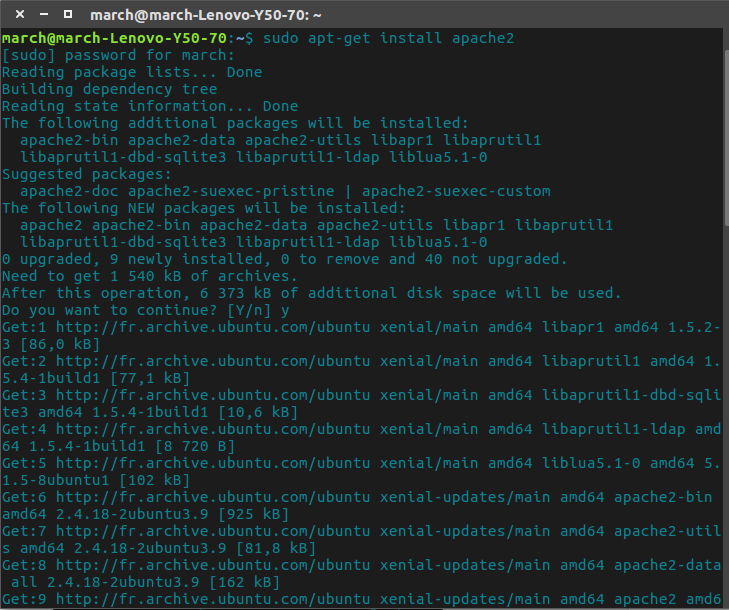
\includegraphics[width=.68 \textwidth]{images/http1}
		\caption{Comando de instalación HTTP apache2.}
		\label{image:http1}
\end{figure}
\FloatBarrier

Una vez que se realizó la instalación de los paquetes correspondientes a dicho servidor, se ejecutó el comando \textbf{sudo systemctl status apache2} con el cual se verificaba que el servidor estuviera activo como se observa en la figura \ref{image:http2}.

\FloatBarrier
\begin{figure}[htbp!]
		\centering
			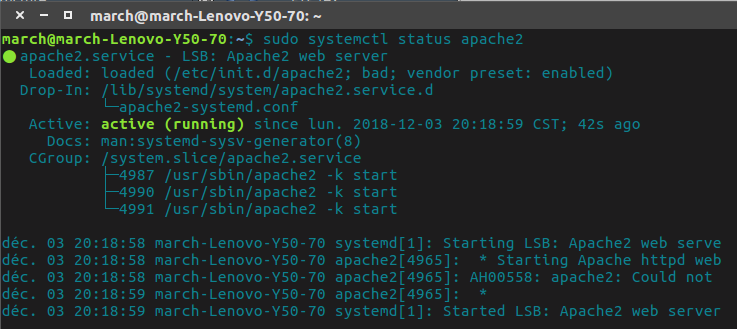
\includegraphics[width=.75 \textwidth]{images/http2}
		\caption{Verificación de status servidor HTTP.}
		\label{image:http2}
\end{figure}
\FloatBarrier

Y una vez que se verifica que su status es activo, se visualiza en terminal la IP de la máquina con el fin de ingresarla en el navegador mediante el cual se obtiene la página de inicio del servidor de Apache (figuras \ref{image:http3} y \ref{image:http4}).

\FloatBarrier
\begin{figure}[htbp!]
		\centering
			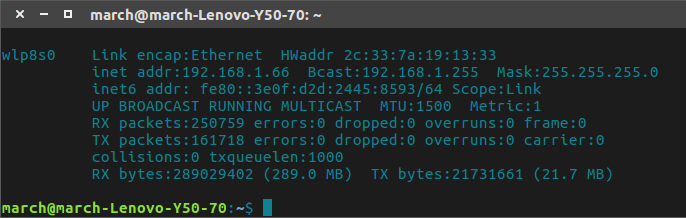
\includegraphics[width=.75 \textwidth]{images/http3}
		\caption{Visualización de ip.}
		\label{image:http3}
\end{figure}
\FloatBarrier

\FloatBarrier
\begin{figure}[htbp!]
		\centering
			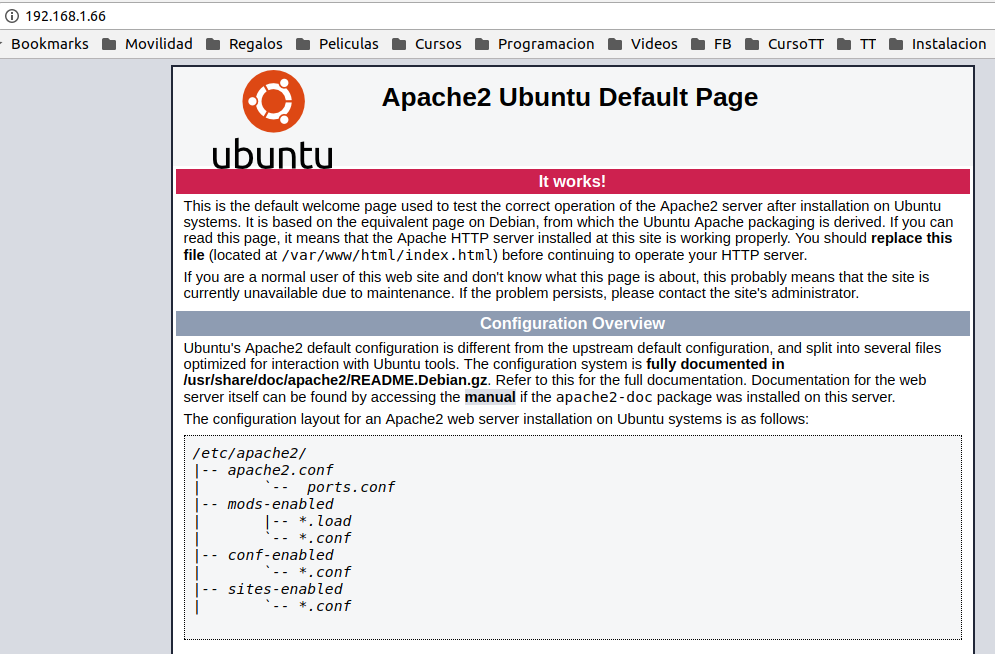
\includegraphics[width=.75 \textwidth]{images/http4}
		\caption{Página de Apache2 en el navegador.}
		\label{image:http4}
\end{figure}
\FloatBarrier

\subsection{Funcionamiento}
Ya que se ha realizado correctamente toda la instalación del servidor, se prueba este mediante el sensor HTTP. Al ejecutar el programa de python, nuevamente nos aparece el menú de opciones y se selecciona la opción 2 la cual nos despliega la información perteneciente a dicho servidor como lo es el tiempo de respuesta, los bytes recibidos y la velocidad del ancho de banda (figura \ref{image:http5}).

\FloatBarrier
\begin{figure}[htbp!]
		\centering
			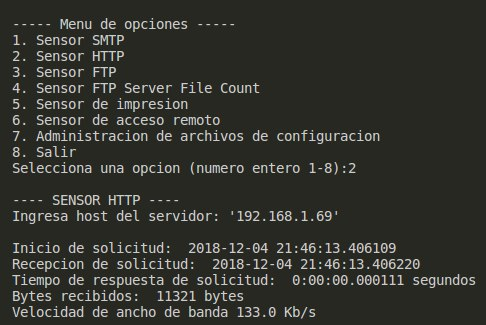
\includegraphics[width=.6\textwidth]{images/http5}
		\caption{Sensor de monitoreo HTTP.}
		\label{image:http5}
\end{figure}
\FloatBarrier

La imagen de la figura \ref{image:http6}, muestra el código del funcionamiento de esta sección en el cual se solicita primero el host del servidor HTTP y posteriormente se realiza una petición en este caso GET, misma que puede cambiar por POST o cualquier otra que se desee y con base en esto, se obtienen el tiempo de respuesta de la solicitud, los bytes transmitidos y la velocidad del ancho de banda.
\FloatBarrier
\begin{figure}[htbp!]
		\centering
			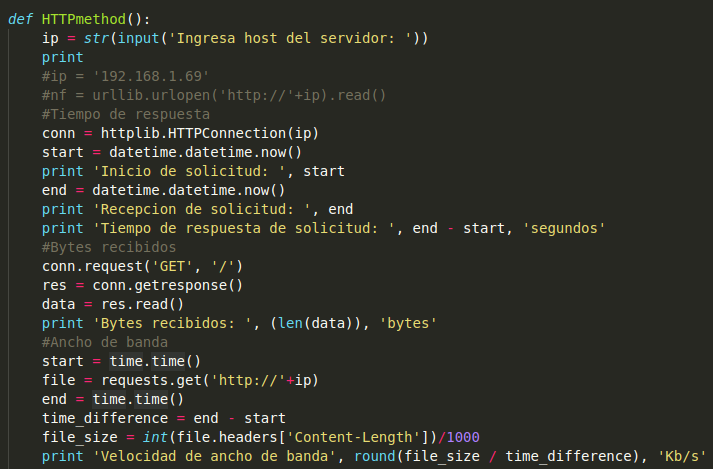
\includegraphics[width=.75\textwidth]{images/http6}
		\caption{Código de sensor de monitoreo HTTP.}
		\label{image:http6}
\end{figure}
\FloatBarrier
